\chapter{The Stages of Life}\label{ch:g3:stages-of-life}

Line up a family photograph: the baby on Grandma's \omterm{def:g1:my-body:joint}{knee}, the
schoolchild missing two front teeth, the teenage cousin suddenly
taller than his mother, the parents, Grandma herself. One family,
one afternoon --- and the whole human \omterm{def:g2:born-grow-die:cycle}{life cycle} sitting on one
sofa. This year we look closely at those stages, and at how
growth itself can be measured.

\section{The stages of a human life}

\begin{definition}[The stages of human life]\label{def:g3:stages-of-life:stages}
A human life passes through stages:
\begin{enumerate}
  \item the \emph{baby}\index{baby} (roughly the first two
        years): fastest growth of all, first teeth, first steps,
        first words;
  \item the \emph{child}\index{child}: steady growth, \omterm{prop:g2:teeth-and-eating-well:sets}{baby teeth}
        traded for \omterm{prop:g2:teeth-and-eating-well:sets}{adult teeth}, learning of every kind;
  \item the \emph{adolescent}\index{adolescent}: a new burst of
        fast growth, and the body changing from a child's into an
        adult's;
  \item the \emph{adult}\index{adult}: growth in height over;
        adults can become parents;
  \item \emph{old age}\index{old age}: hair whitens, \omterm{def:g1:the-five-senses:sense}{skin}
        wrinkles, strength slowly declines --- the natural last
        stage of the cycle.
\end{enumerate}
\end{definition}

\begin{example}[Reading the sofa]\label{ex:g3:stages-of-life:sofa}
On the family sofa: the baby (stage 1), the gap-toothed
schoolchild (stage 2 --- the changeover of
\cref{ch:g2:teeth-and-eating-well} in full swing), the
sixteen-year-old cousin (stage 3, mid-burst), the parents (stage
4), Grandma (stage 5). Five stages, one family.
\end{example}

\begin{omfigure}
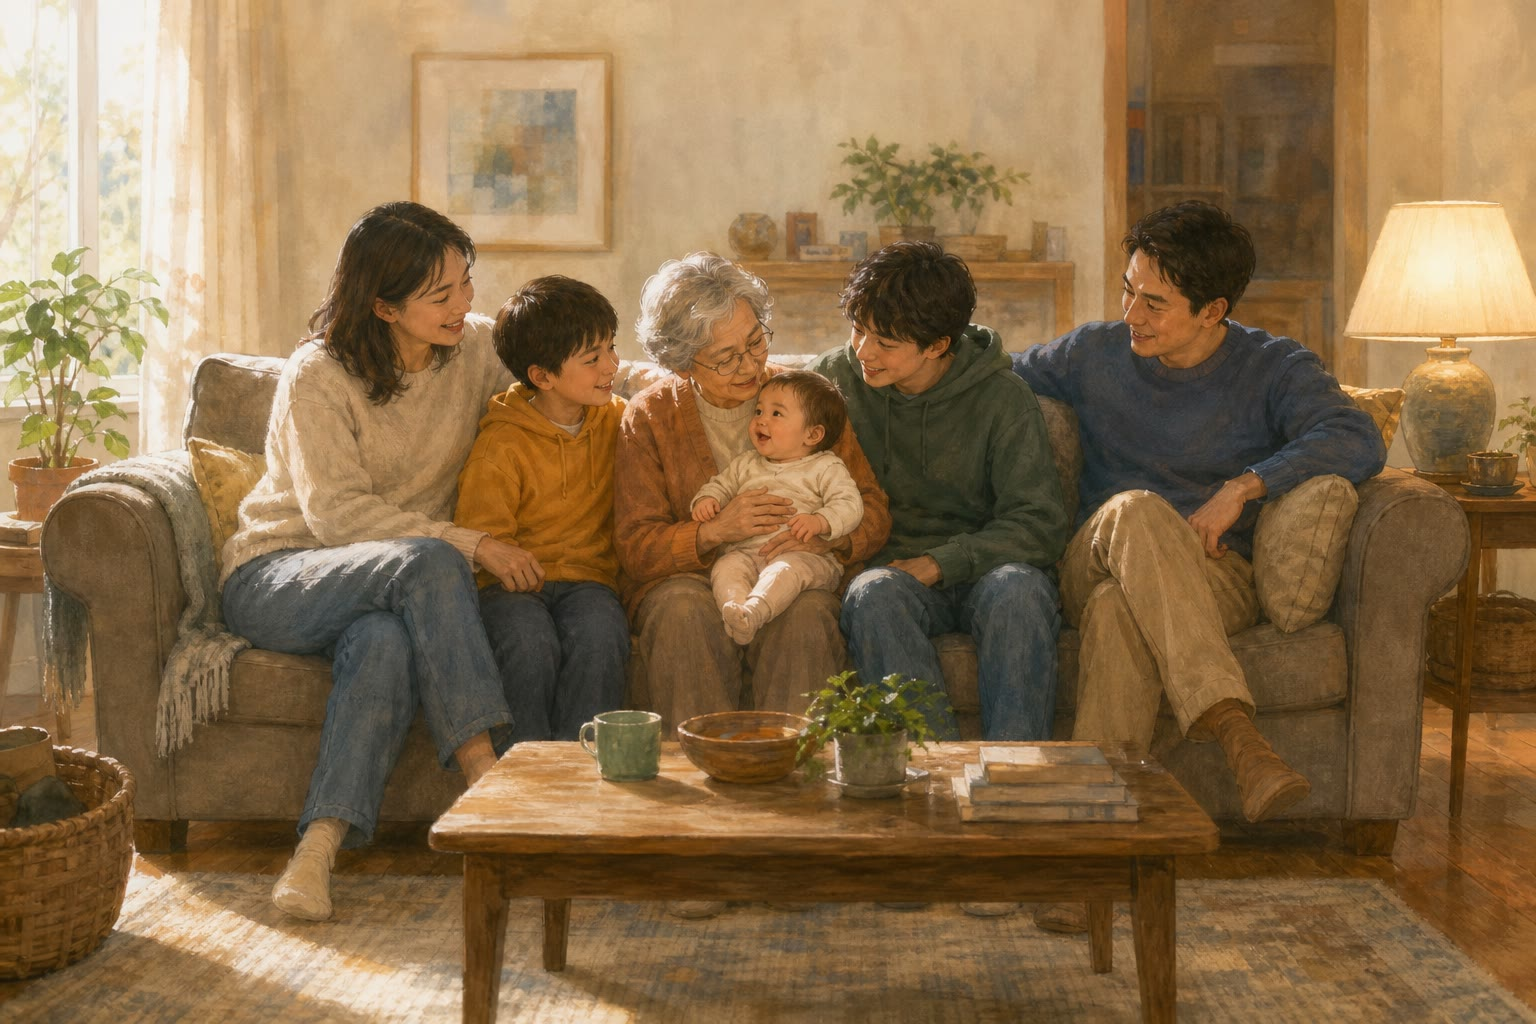
\includegraphics[width=0.62\linewidth]{images/book1/ai/g3-stages-family.jpg}

{\small The whole cycle on one sofa: baby, child, \omterm{def:g3:stages-of-life:stages}{adolescent},
\omterm{def:g3:stages-of-life:stages}{adults}, grandmother.}
\end{omfigure}

\begin{remark}[Growing is not steady]\label{rem:g3:stages-of-life:bursts}
Growth has a rhythm: very fast for the baby --- height roughly
half as much again in the first year --- slower and steady
through childhood, fast again for the \omterm{def:g3:stages-of-life:stages}{adolescent}, then over. Two
bursts with a calm stretch between: that is the normal shape of
growing up.
\end{remark}

\section{Measuring growth}

\begin{definition}[Growth chart]\label{def:g3:stages-of-life:chart}
A \emph{growth chart}\index{growth chart} is a record of height
(or weight) measured again and again over time --- the door-frame
marks of \cref{ch:g1:my-body}, made regular and dated. Doctors
keep one for every child.
\end{definition}

\begin{omfigure}
\begin{tikzpicture}
\begin{axis}[omaxis,
    width=9.2cm, height=6cm,
    xlabel={age (years)}, ylabel={height (cm)},
    xmin=0, xmax=22.5, ymin=0, ymax=190,
    xtick={0,5,10,15,20},
    ytick={50,100,150},
    ]
  \addplot[very thick, omDef, smooth] coordinates {
    (0,50) (1,75) (2,87) (4,102) (6,115) (8,127) (10,138)
    (12,150) (14,165) (16,175) (18,178) (20,178)
  };
\end{axis}
\end{tikzpicture}

{\small A \omterm{def:g3:stages-of-life:chart}{growth chart} from \omterm{def:g2:born-grow-die:cycle}{birth} to adulthood: steep for the
baby, steady for the child, steep again for the \omterm{def:g3:stages-of-life:stages}{adolescent}, then
flat --- growth is over.}
\end{omfigure}

\begin{example}[Reading the chart]\label{ex:g3:stages-of-life:reading}
On the chart, the line climbs about $\qty{25}{cm}$ in the very
first year --- and only about $\qty{6}{cm}$ a year through
childhood. The two steep parts are the two bursts of
\cref{rem:g3:stages-of-life:bursts}; the flat end says the \omterm{def:g3:stages-of-life:stages}{adult}
has stopped growing taller.
\end{example}

\begin{method}[Keeping your own growth chart]\label{met:g3:stages-of-life:keep}
\begin{enumerate}
  \item Measure height carefully (the wall-and-book way of the
        earlier years), always without shoes;
  \item write the date and the height in a notebook, or mark the
        door frame and date the mark;
  \item measure again every few months --- regularity matters
        more than frequency;
  \item to see the story, plot the points: age along the bottom,
        height up the side, like the figure.
\end{enumerate}
\end{method}

\section{Animals and plants have stages too}

\begin{proposition}[Stages across the living world]\label{prop:g3:stages-of-life:animals}
Every \omterm{def:g1:living-or-not:living}{living thing} passes through stages of its own version of
the cycle --- young, \omterm{def:g3:stages-of-life:stages}{adult}, \omterm{def:g3:stages-of-life:stages}{old age}. The young stage may look
like the \omterm{def:g3:stages-of-life:stages}{adult} (the kitten, the foal) or nothing like it (the
tadpole, the \omterm{ex:g2:animals-grow-up:butterfly}{caterpillar} of \cref{ch:g2:animals-grow-up}); a
\omterm{def:g1:plants-around-us:plant}{plant}'s stages run \omterm{def:g2:from-seed-to-plant:seed}{seed}, \omterm{prop:g2:from-seed-to-plant:cycle}{seedling}, young \omterm{def:g1:plants-around-us:plant}{plant}, flowering \omterm{def:g3:stages-of-life:stages}{adult}.
What none of them can do is skip a stage or run them backward.
\end{proposition}
\admitted

\begin{example}[How fast, how slow]\label{ex:g3:stages-of-life:speeds}
The speeds differ enormously. A fly is \omterm{def:g3:stages-of-life:stages}{adult} in weeks; a cat in
about a year; a human in nearly twenty years; an oak takes
several tens of years before its first acorns. Slow or fast, the
order of the stages never changes.
\end{example}

\begin{remark}[Old age is a stage, not a defect]\label{rem:g3:stages-of-life:oldage}
White hair and wrinkles are not an illness: they are the body's
last stage, as natural as the baby's first teeth. In many
species, and in human families, the old ones carry what the
young most need --- experience.
\end{remark}

\section{Exercises}

\begin{exercise}[$\star$]\label{exo:g3:stages-of-life:1}
Name the five stages of a human life, in order.
\end{exercise}

\begin{exercise}[$\star$]\label{exo:g3:stages-of-life:2}
At which stage: (a) do the \omterm{prop:g2:teeth-and-eating-well:sets}{baby teeth} fall out? (b) can a person
become a parent? (c) is growth the fastest of the whole life?
\end{exercise}

\begin{exercise}[$\star$]\label{exo:g3:stages-of-life:3}
What are the two bursts of growth, and what lies between them?
\end{exercise}

\begin{exercise}[$\star$]\label{exo:g3:stages-of-life:4}
On the \omterm{def:g3:stages-of-life:chart}{growth chart}, how can you tell from the line alone that an
\omterm{def:g3:stages-of-life:stages}{adult} has stopped growing?
\end{exercise}

\begin{exercise}[$\star$]\label{exo:g3:stages-of-life:5}
Using the chart, about how many centimetres does the line climb
between ages $6$ and $8$? And in the single first year?
\end{exercise}

\begin{exercise}[$\star$]\label{exo:g3:stages-of-life:6}
Why must height always be measured without shoes, the same way
each time? What could go wrong otherwise?
\end{exercise}

\begin{exercise}[$\star$]\label{exo:g3:stages-of-life:7}
Give the stages of an oak tree's life, from acorn to old tree.
\end{exercise}

\begin{exercise}[$\star$]\label{exo:g3:stages-of-life:8}
Try it: start the \omterm{def:g3:stages-of-life:chart}{growth chart} of
\cref{met:g3:stages-of-life:keep} for yourself, with today's
first point. Which stage of \cref{def:g3:stages-of-life:stages}
are you in --- and which burst is still ahead of you?
\end{exercise}

\begin{exercise}[$\star\star$]\label{exo:g3:stages-of-life:9}
A fly, a cat, a human and an oak run the same stages at very
different speeds. Order them from fastest to slowest to reach
adulthood --- and say what all four orders of stages have in
common.
\end{exercise}

\begin{exercise}[$\star\star$]\label{exo:g3:stages-of-life:10}
Tom, aged $9$, measures himself twice in one month and finds
``no growth at all''. Should he worry? Answer with
\cref{rem:g3:stages-of-life:bursts} and the shape of the chart
at his age.
\end{exercise}
